\documentclass[border=0pt]{standalone}
\usepackage[T1]{fontenc}
\usepackage{lmodern}
\usepackage{pgfplots}
\usepgfplotslibrary{groupplots}
\pgfplotsset{compat=1.18}
\definecolor{f02sg}{HTML}{0072B2}
\definecolor{f02arpls}{HTML}{D55E00}
\begin{document}
\begin{minipage}{181.86mm}
\centering
{\bfseries\fontsize{10}{12}\selectfont P08-F02 Source-selected CNN / M06 combined predictions per physical sample / Sensitivity (S)}\par\vspace{6mm}
% semantic SHA-256: 4c3507299219d2ce29fd9a2a58f030be1b778fd9bbceb756756ca16d12f674f7
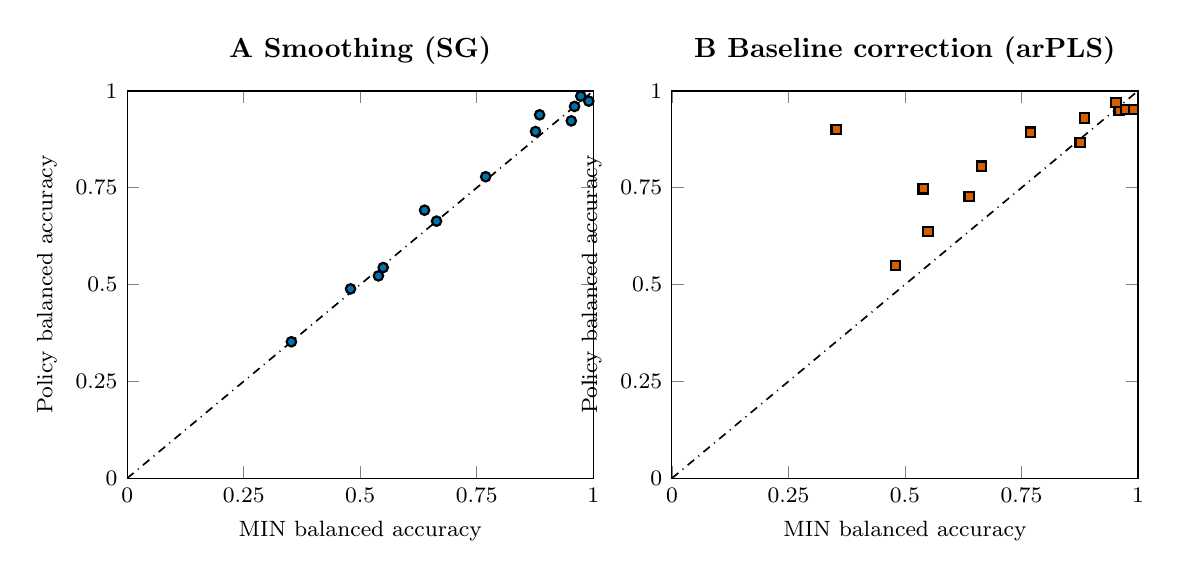
\begin{tikzpicture}
\begin{groupplot}[
  group style={group size=2 by 1, horizontal sep=10mm, vertical sep=6mm},
  width=75mm, height=65mm,
  xmin=0, xmax=1, ymin=0, ymax=1,
  xtick={0,0.25,0.5,0.75,1}, ytick={0,0.25,0.5,0.75,1},
  tick label style={font=\fontsize{8}{9}\selectfont},
  label style={font=\fontsize{8}{9}\selectfont},
  title style={font=\bfseries\fontsize{10}{12}\selectfont},
  xlabel={MIN balanced accuracy}, ylabel={Policy balanced accuracy},
]
\nextgroupplot[title={A  Smoothing (SG)}]
\addplot[black, dash dot, line width=0.6pt, samples=2, domain=0:1, forget plot] {x};
\addplot[only marks, mark=*, mark size=1.7pt, color=f02sg, mark options={draw=black,line width=0.8pt}] coordinates {(0.5391534391534393,0.5224867724867724) (0.5493386243386242,0.544047619047619) (0.663888888888889,0.663888888888889) (0.885,0.9383333333333332) (0.96,0.96) (0.35238095238095235,0.35238095238095235) (0.9733333333333333,0.9866666666666667) (0.9904761904761905,0.9738095238095237) (0.47936507936507927,0.48888888888888893) (0.638095238095238,0.692063492063492) (0.9530303030303031,0.9227272727272726) (0.8761904761904763,0.8952380952380953) (0.7692592592592592,0.7785185185185186)};
\nextgroupplot[title={B  Baseline correction (arPLS)}]
\addplot[black, dash dot, line width=0.6pt, samples=2, domain=0:1, forget plot] {x};
\addplot[only marks, mark=square*, mark size=1.7pt, color=f02arpls, mark options={draw=black,line width=0.8pt}] coordinates {(0.5391534391534393,0.7472222222222222) (0.5493386243386242,0.6370370370370371) (0.663888888888889,0.8055555555555556) (0.885,0.9299999999999999) (0.96,0.9504761904761903) (0.35238095238095235,0.9) (0.9733333333333333,0.9523809523809523) (0.9904761904761905,0.9523809523809523) (0.47936507936507927,0.5492063492063493) (0.638095238095238,0.7269841269841268) (0.9530303030303031,0.9696969696969697) (0.8761904761904763,0.8666666666666668) (0.7692592592592592,0.8933333333333333)};
\end{groupplot}
\end{tikzpicture}
\par\vspace{4pt}
{\fontsize{8}{10}\selectfont RQ-S01: preprocessing and chemical identification. Source-only selection/calibration; selected CNN identity fixed across policies. SG = impulse replacement, smoothing, minmax; arPLS = impulse replacement, baseline correction, minmax. MIN = minimal minmax. Primary: equal contexts within domain, then equal domains. Pooled-fold sensitivity reconstructs each four-fold prediction set before scoring. M01 individual-spectrum predictions; M06 combined predictions per physical sample. M06 averages model probabilities within sample/instrument then equally across instruments, never input spectra or hard labels. 598 original spectra / 69 physical samples / 10 instruments; 557 spectra in 13 held station/instrument domains, 260 contexts. Per-domain independent support in the CSV/table. D1..D13 are lexicographic station/instrument domains, not samples. Diagonal y=x; the 520 points across all panels are paired domain measurements, not 520 independent observations. Claim limit: cannot establish causal background removal or new-instrument performance; no error bars, no significance stars.}\par
\end{minipage}
\end{document}